\section{WSD Learning Rate Scheduler}
\label{sec:wsdlrs}
\subsection{Analysing Cosine LRS}

The current commonly used learning rate strategy is the Cosine LRS~\citep{kaplan2020scaling, hoffmann2022training, rae2021scaling, touvron2023llama, bai2023qwen, almazrouei2023falcon}, which gradually decreases the learning rate following a cosine curve after it reaches its maximum after the warmup stage. 

A key hyper-parameter in the Cosine LRS is the step $T$ at which Cosine decreases to the minimum for the first time. \uline{Typically, $T$ is set to the total training step $S$ for training with a predefined training step.} Generally, it is believed that the learning rate should be high to enable sufficient exploration. We try $Cosine(T)$ and $CosineLoop(T)$ LRS, following the formula shown in Appendix~\ref{app:lrsequ}. The result can be seen in Figure~\ref{fig:cosine_lr}. We can see that when the training step is $S=20N, 40N, 60N, 80N$, the lowest loss is always achieved by the $Cosine(T)$ where $T = S$. Both $T<S$ and $T>S$ are not optimal. 

We hypothesize that the Cosine LR performs exceptionally well when $T = S$ because of the following two reasons: 

(1) Cosine LRS with $T = S$ has a longer duration of \textit{high learning rate} training compared to $T < S$ and other LRS such as Linear LRS. \uline{This high learning rate might help the model find a better global optimum.}

(2) \uline{Cosine LRS with $T = S$ has a more thorough learning rate decay phase compared to Cosine LRS with $T > S$ and Constant LRS.} This learning rate decay may involve unique training dynamics that enable the model to find a better local optimum.

\subsection{WSD LRS}

\uline{In light of the above perspective, we propose to explicitly divide the training stage into the high learning rate stage and learning rate decay stage.} We name it as the Warmup-Stable-Decay (WSD) LRS.  Especially, the WSD LRS contains three stages: \uline{the warmup stage} (whose end step is denoted by $W$), \uline{the stable training stage} (whose end step is denoted by $T$), and \uline{the remaining decay stage}. The function form of WSD is:

\vspace{-2mm}
\begin{equation}
    WSD(T; s) = \begin{cases}
       & \frac{s}{W} \eta, \quad s<W\\
       & \eta, \quad W < s < T \\
       & f(s-T)\eta,\quad T < s < S\\
    \end{cases}
\end{equation}

where $0< f(s-T)\leq 1$ is a decreasing function about $s$, $\eta$ is the maximum learning rate.

\subsection{Experiments}
\label{sec:wsd_experiments_continoustrain}

\textbf{Loss Decreases Dramatically in Decay Stage. } As shown in Figure~\ref{fig:wsd_diff_dcay}, in the decay stage, as the learning rate begins to decrease, the loss experiences a significant rapid decline and quickly decreases to be equal to or lower than the Cosine LRS at step $T=S$. \uline{At the same time, we can reuse the model before decay and continue training with the previous high learning rate.} \uline{After more steps of training $S'$, we can also perform annealing to achieve the same loss as the Cosine LRS at $Cosine(S')$.} This verifies our assumption that the training stage can be explicitly split into the stable training and decay stages.

\begin{figure}[htbp]
    \centering
    \begin{minipage}{0.48\linewidth}
        \centering
        \includegraphics[width=1.05\linewidth]{Fig/WSD_diff_dcay.pdf}
        \caption{ Model training loss has a sudden decrease in the decay stage of WSD LRS. }
        \label{fig:wsd_diff_dcay}
        \vspace{0.47cm}
    \end{minipage}
    \hfill % This adds a little space between the two figures
    \begin{minipage}{0.48\linewidth}
        \centering
    \includegraphics[width=1.05\linewidth]{Fig/continuous_train.pdf}
    \caption{Continous training a 0.036B model can match the performance of 0.17B model with an acceptable increase in training compute.}
    \label{fig:continuoustrain}
    \end{minipage}
\end{figure}

\textbf{10\% Steps are Enough.} \uline{From the two-stage training perspective, shortening the decay stage will greatly benefit the fast test of different model checkpoints of stable training.} Also shown in Figure~\ref{fig:wsd_diff_dcay}, among all three stable training checkpoints in 40N, 60N, and 80N training data, having a decay of 10\% of the total tokens is sufficient to achieve the best results, while a decay of 2.5\% of total tokens falls short. \uline{Therefore, in the subsequent training experiments, we use a decay of about 10\% to ensure full convergence.}

\textbf{Effective Data Scaling with WSD LRS.} With WSD LRS, we can continuously train the LM to extreme convergence. In Figure~\ref{fig:continuoustrain}, the green lines represent 0.036B models trained with different stable training tokens. Despite the last point of the 0.036B series being trained with many more tokens than Chinchilla Optimal~\citep{hoffmann2022training}, it still has space for performance improvement. 

\definecolor{darkgreen}{rgb}{0.0, 0.5, 0.0}

To find the limit of continuously training this fixed-sized LM, we estimate how the model's optimal performance changes with its computation during continuous training. By optimal performance, we mean the loss of training token $D$ is achieved by ${WSD}(D, 0.1D)$. With a series of $D$, the losses will form the optimal loss envelope. Due to uncertainty about the function form of the loss envelope, we try two fitting formulas: (1) exponential: $L(C) = \alpha e^{-\beta C} + L_0$ and (2) power-law: $L(C) = \beta C^{-\alpha} + L_0$. The fitting results for both functions are in Appendix~\ref{app:fittingdatascaling}. We find that the power-law form fits better (similar to the Cosine LRS~\citep{kaplan2020scaling}). In Figure~\ref{fig:continuoustrain}, the fitted curve is shown in \textcolor{darkgreen}{green} dotted lines. To intuitively estimate and comprehend the effect of continuous training such a fixed-sized model, we also trained a 0.17B model with $WSD(40N, 4N)$, which is shown in \textcolor{pink}{pink} in Figure~\ref{fig:continuoustrain}.  We can see that a 0.036B model can match the performance of a 0.17B model with an acceptable increase ($\sim 4$ times) in training compute while saving a lot of inference computation~\citep{sardana2023beyond} (saving $\sim 5$ times per inference call), indicating a better inference-compute-optimal setting~\citep{sardana2023beyond}.




% To sum up, the WSD strategy has the following two advantages:
% \begin{enumerate}
% \item The model can be trained continuously without a predefined number of tokens. Whenever the model needs to be used at step $S'$, a quick decay stage can be conducted to get the best loss that is comparable to $Cosine(T)$ that has $T = S'$.
% \item There are explicitly distinguishable training stages, which facilitate the use of different data strategies, which will be described in detail in~\ref{sec:trainingstrategy}.
% \end{enumerate}


\subsection{Analysis of the Decay Stage}
In this section, we provide a brief analysis of the loss drop in the decay stage, examining it through the prisms of checkpoint updates and gradient information.  We calculate the maximum weight element update $max_{ij} (W_{ij}^{(t+1)} - W_{ij}^{(t)})$ across all weight matrices in the MiniCPM-2.4B (Introduced in Section~\ref{sec:model}). As depicted in Figure~\ref{fig:appmaxdiff}, the updates exhibit a robust correlation with the learning rate's magnitude. Notwithstanding the illustration of the two submodules (gate\_proj and q\_proj module of the 25th layer), this pattern is prevalent across every layer and submodule within the network. This observation may not be trivial: the model checkpoints experience significant updates preceding the learning rate's decay, yet the loss exhibits minimal reduction. Conversely, during the decay stage, despite less pronounced weight alterations, there is an accelerated decrease in loss.  


\begin{figure}[htbp]
    \centering
    % First minipage for the first figure
    \begin{minipage}{0.48\linewidth}
        \centering
        \includegraphics[width=1.0\linewidth]{Fig/gate_proj_projection_vs_rank_25.pdf}
    \end{minipage}
    \hfill % This adds a little space between the two figures
    % Second minipage for the second figure
    \begin{minipage}{0.48\linewidth}
        \centering
        \includegraphics[width=1.0\linewidth]{Fig/q_proj_projection_vs_rank_25.pdf}
    \end{minipage}
     \caption{Max Difference of Checkpoints.}
        \label{fig:appmaxdiff}
\end{figure}


Further examination of the gradient data is undertaken by training a 0.2B model, meticulously recording every step gradient information, and evaluating the differences between consecutive steps, thereby providing an approximation of second-order gradient information. We treat the gradient at step $t$ as a flattened vector $\mathbf{g}^{(t)}$, and the parameter (also flattened as a vector $\mathbf{x}^{(t)}$ ) update between step $t$ and $t+1$ is $\mathbf{v}^{(t)} = \mathbf{x}^{(t+1)} - \mathbf{x}^{(t)}$. The gradient norm take the $L2$ norm of the gradient $\Vert\mathbf{g}^{(t)} \Vert$, gradient inner product is $\mathbf{g}^{(t+1)} \cdot \mathbf{g}^{(t)}$, the cosine of the gradient's angle is given by $\frac{\mathbf{g}^{(t+1)} \cdot \mathbf{g}^{(t)}}  {\Vert\mathbf{g}^{(t+1)} \Vert \Vert\mathbf{g}^{(t)} \Vert}$. Imaging the optimization process as a trajectory over a high-dimension manifold, first order directional derivative along the trajectory is computed as $D_1 = \frac{\mathbf{g}^{(t+1)} \cdot \mathbf{v}^{(t)}}{\|\mathbf{v}^{(t)}\|}
$, and the second order directional derivative is $D_2 = \frac{(\mathbf{g}^{(t+1)} - \mathbf{g}^{(t)}) \cdot \mathbf{v}^{(t)}}{\|\mathbf{v}^{(t)}\|^2}
$. $D_1, D_2$ enables an approximate estimation of the loss curvature on the trajectory, $K = \frac{|D_2|}{(1 + D_1^2)^{\frac{3}{2}}}$. The results of these statistics over time are shown in Figure~\ref{fig:grad}. We can see that the gradient norm diminishes during the decay phase, and upon commencement of this stage, the cosine between gradients predominantly assumes positive values, suggesting that in the decay phase, model parameters undergo consistent changes across steps. Concerning directional derivatives, it is remarkable that the first-order directional derivative diminishes exponentially with each step, aligning closely with the learning rate, while the second-order directional derivative exhibits a slight increase in magnitude. The curvature of the loss function also increases by a magnitude, indicating the proximity to a local optimum. These findings potentially offer a deeper insight into the shape optimization space, a subject reserved for future exploration.


\begin{figure}[htbp]
    \centering
    % First minipage for the first figure
        \centering
        \includegraphics[width=1.0\linewidth]{Fig/grad.pdf}
     \caption{Gradient statistics over the training of a 0.2B model using WSD LRS. The exponential decay stage begins at 8000 steps.}
        \label{fig:grad}
\end{figure}



\subsection{Measuring the Scaling Law with WSD LRS}
\label{scalinglawwsdlrs}
Scaling laws serve as a fundamental guiding principle in the development of LLMs. Although these scaling laws exhibit variability in specific coefficients due to diverse configurations across model series, the compute optimal data-to-model ratio remains a meaningful metric across different scaling law functions, which ``marginalizes`` out the specific value of loss. Regarding this ratio, \cite{kaplan2020scaling} posit that a tenfold increase in model scale should equate to a singlefold increase in data scale. Conversely, \cite{hoffmann2022training} argue for the same scaling rate between model size and data size. What's more, current models such as LLama 2~\citep{touvron2023llama}, train much more data than what \cite{hoffmann2022training} claims, still yielding considerable performance gain. Indicating a higher data-to-model ratio. 

This unaddressed uncertainty stems from the challenges inherent in training multiple models of varying sizes and data sizes in traditional scaling experiments. Previously, if the average cost of training one model size on one data size is $C$, then conducting the scaling experiments with $m$ model sizes and $m$ data sizes takes approximately $O(m^2)C$. 


In this section, we introduce the utilization of the WSD scheduler as an effective approach to explore the scaling law with linear cost ($O(mC)$).
Since the WSD scheduler has the advantage of arriving at the optimal loss of Cosine LRS after decaying from stable stage checkpoints of any step, we are now able to precisely measure the optimal scaling properties without re-training the models from scratch to different amounts of tokens, thus making the scaling law measurement much more efficient along the data axis.

We measure the scaling law along the data and model axes by training SLMs of 6 sizes ranging from 0.04B to 2B, each with 6 decayed models starting from the checkpoint of $10N$ to $60N$ data during the stable training stage. The final loss is evaluated on five held-out evaluation datasets. To potentially compare the loss when the model uses different tokenizers, we take the average of loss by a number of bytes instead of a number of tokens, following~\cite{achiam2023gpt}. The final loss of each pair of data size and model size is shown in the blue lines in Figure~\ref{fig:individual_task_datascalinglaw}. 

Then we fit the losses with model size $N$ and data size $D$ following ~\cite{hoffmann2022training} using scipy \texttt{curvefit} function:

\begin{equation}
    L(N, D) = C_NN^{-\alpha} + C_DD^{-\beta} + L_0
\label{equ:scalinglaw}
\end{equation}

The fitted curve along the data axis for each dataset and each checkpoint are shown in orange lines in Figure~\ref{fig:individual_task_datascalinglaw}.
Then we have the optimal model size $N_{opt}$, dataset size $D_{opt}$, given a fixed amount of compute $C=6ND$~\citep{rae2021scaling} as: 

\begin{equation}
    \frac{N_{opt}}{D_{opt}} = K^2\left(\frac{C}{6}\right)^{\eta},
\label{equ:computeoptimal}
\end{equation}

where $K = (\frac{\alpha C_N}{\beta C_D})^{\frac{1}{\alpha + \beta}} $, and $\eta=\frac{\beta-\alpha}{\alpha+\beta}$. The derivation of $N_{opt}$ closely follows ~\cite{hoffmann2022training} by substituting $D$ with $\frac{C}{6N}$ in Equation~\ref{equ:scalinglaw}, and minimize $L(N)$ given $C$.  A similar way is adopted for $D_{opt}$. 
From Equation~\ref{equ:computeoptimal}, when $\alpha = \beta$, $N_{opt}/D_{opt}$ is a constant, supporting ~\cite{hoffmann2022training}'s claim, and when $\alpha < \beta$, we should emphasize more on parameter scaling~\citep{kaplan2020scaling}, and vise versa. 

In our experiments, the fitted relationship between loss and $N, D$ is shown in the contour plot of equal loss in Figure~\ref{fig:wsd_optimalscalinglaw}. The equation of fitted scaling law is shown in the first text box in each subplot. We can see that in all evaluation corpora, we have $\beta < \alpha$. More specifically, on average, we have $\alpha=0.29, \beta=0.23, K^2 = 0.01, \eta=-0.10$. Since $\alpha$ is slightly larger than $\beta$, this result shows that as the computation scale, we should slightly emphasize more on data scaling than model scaling, which aligns with ~\cite{hoffmann2022training}.

As for the concrete data-to-model ratio $\frac{D_{opt}}{N_{opt}}$,  we notice that there is a huge gap in compute optimal regime between ours and ~\cite{hoffmann2022training} despite that the trend of $\frac{D_{opt}}{N_{opt}}$' with compute $C$ is aligned between ours and theirs. Specifically, the data size should be 192 times larger than the model size on average, as opposed to 20 times in ~\cite{hoffmann2022training}. We note that this aligns with the observation in Section~\ref{sec:wsd_experiments_continoustrain} and Figure~\ref{fig:continuoustrain}.

With respect to the large deviation from Chinchilla Optimal $\frac{N_{opt}}{D_{opt}}$, we notice that their scaling experiment was conducted in a not very recent configuration. To compare with more recent configuration such as Llama2~\citep{touvron2023llama}, we extract the training loss data from Llama2 paper (left part) in Appendix Figure~\ref{fig:llamascaling} and estimate the compute optimal $\frac{D_{opt}}{N_{opt}}$ in their paper using the right part of Figure~\ref{fig:llamascaling}. Since they use Cosine LRS, the loss is not optimal in the middle of the training, depicted by the concave curve during training in the right figure of Figure~\ref{fig:llamascaling}. We fill the concave part with a straight line to estimate the optimal loss envelope if they had used the WSD LRS. After that, the compute model size should roughly be the regime in which a model's loss curve is about to intersect with a larger model's loss curve. With this intuition, the 13B model is about to intersect with the 34B model at $10^5$ EFlops ($10^18$ Flops), and the 34B model is about to intersect with the 70B model at $5\times 10^5$ EFlops. Therefore, we estimate the $\frac{D_{opt}}{N_{opt}}$ to be roughly $\frac{5\times 10^5}{6\times 34^2} \sim \frac{10^5}{6\times 13^2} $, which is $70 \sim 100$. Therefore, under this approximate comparison, their data-model ratio is closer to ours. And our configuration can absorb more data into a smaller model compared to previous ones. However, we note that the above estimates are only a rough one. 

A larger data-to-model ratio means that we can absorb more data into a smaller model than we previously thought, which is more efficient for inference and deployment. We hope WSD LRS will help more researchers explore $L(N, D)$ with less effort and make the relationship clearer in LLMs.  

% which means that we should scale up more amount of tokens than model sizes, supporting ~\cite{hoffmann2022training}. 
% The derivation is as follow:

% \begin{align}
%     \frac{\mathrm{d} L}{\mathrm{d} N} = 0 give us  N_{opt} = K_N C^{\frac{\beta}{\beta + \alpha}} , \frac{\mathrm{d} L}{\mathrm{d} D} = 0 give us D_{opt} = K_D C^{\frac{\alpha}{\beta + \alpha}}, 
% \end{align}
% where $K_N = (\frac{\alpha C_N}{6^\beta \beta C_D})^{\frac{1}{\alpha + \beta}}, K_D = (\frac{\beta C_D}{6^\alpha \alpha C_N})^{\frac{1}{\beta + \alpha}}$. 



\begin{figure}[!t]
    \centering
    \includegraphics[width=0.92\textwidth]{Fig/lossvscompute_fitted_and_real.pdf}
    \caption{The result of scaling experiments with WSD Scheduler (above) and the fitted scaling curve (below). The x-axis is the computation Flops $C =6ND$, each color of the line represents the same model with different computation Flops. We can see that smaller models are better than larger models when the Flops are small and worse when the Flops are large. Thus models of different sizes will intersect with each other in the plot around the compute optimal regime.}
    \label{fig:wsd_optimalscalinglaw}
\end{figure}




\begin{figure}[!t]
    \centering
    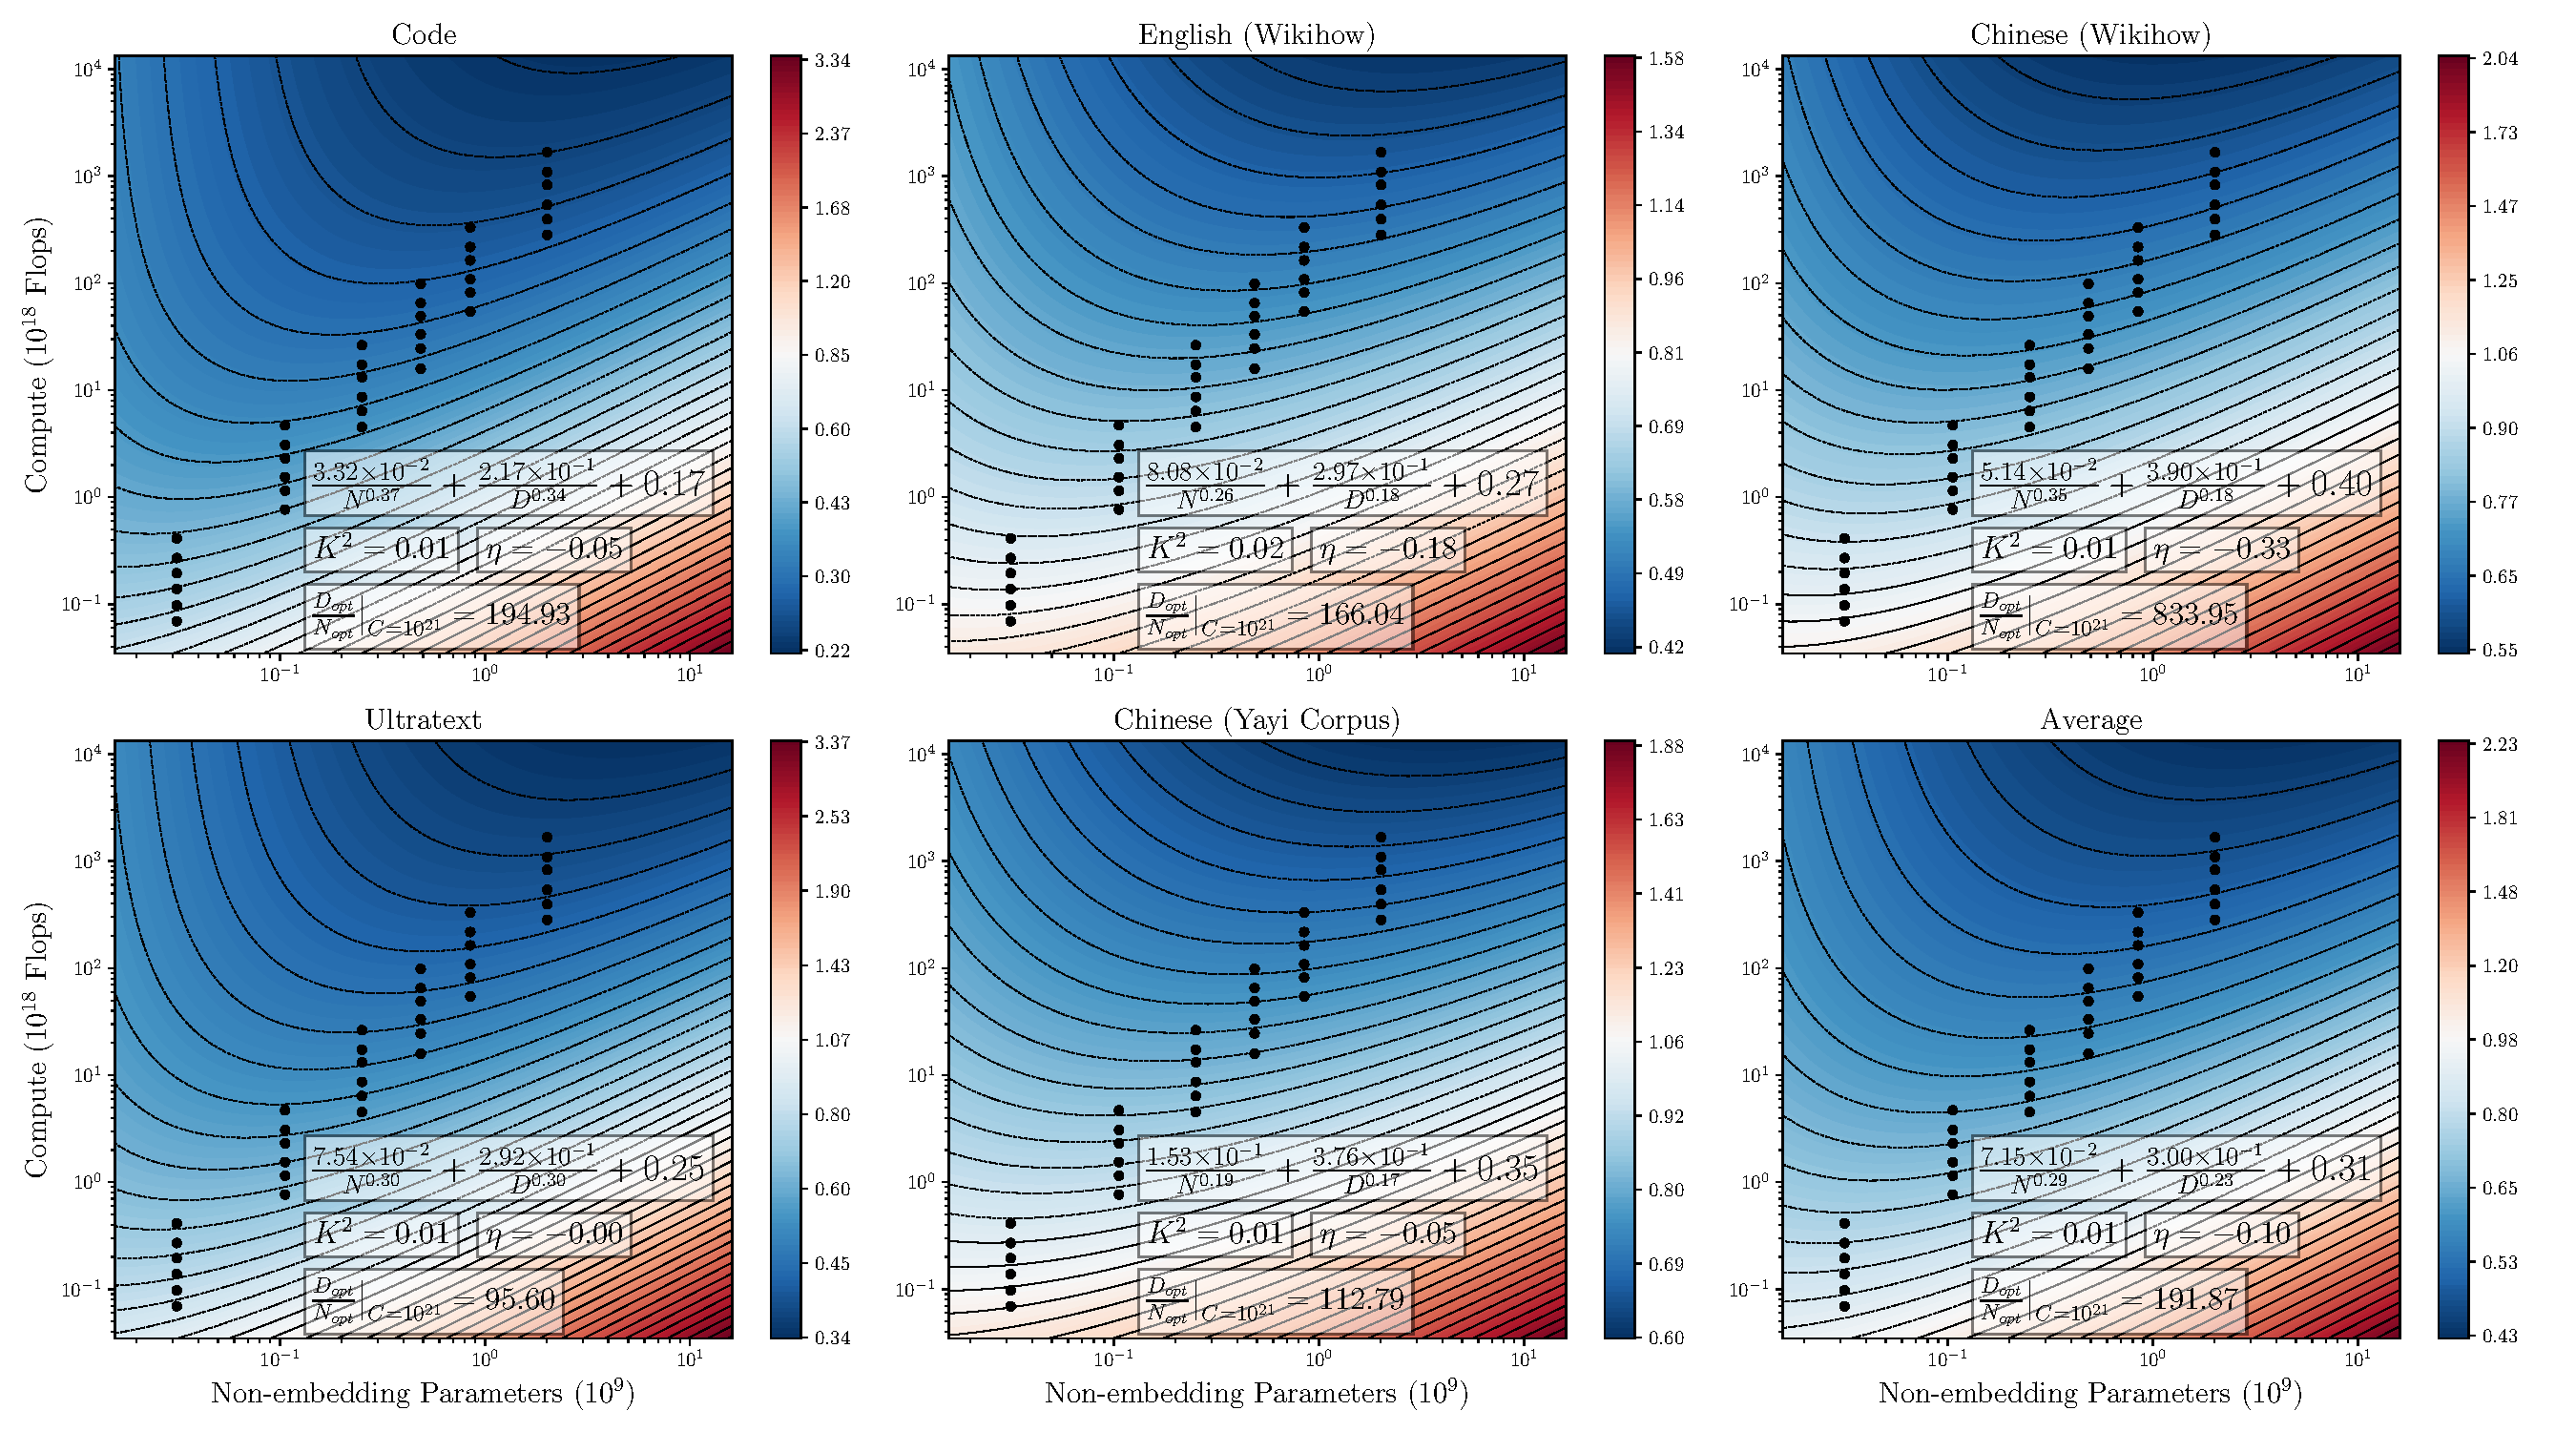
\includegraphics[width=1.0\textwidth]{Fig/wsd_optimal_scaling_law.pdf}
    \caption{The fit result of the scaling experiment with WSD Scheduler. The black dots in a horizontal line denote the decayed checkpoints in different compute within the same model size.}
    \label{fig:wsd_optimalscalinglaw}
\end{figure}

